\section{Experiments}

\subsection{Experiments Setup}
The Ubuntu 16.04 operating system is used in experiments, Python 3.6 programming language, Tensorflow 1.11 and Keras 2.2 frameworks are used to writing programs.
The model is trained using one NVIDIA TITAN X (Pascal) GPU in each experiment.

\subsection{Dataset}
We use the public dataset CelebA\upcite{celeba}, which contains a total of 202,599 facial images, and label 40 attributes for each face.
We align and crop the faces in all images into RGB three-channel images of 128 × 128 pixels and then divide them into training sets, test sets, and verification sets according to the ratio of 8:1:1.
For the 40 attributes in the dataset, we select 4 of them: 'gender', 'skin color', 'hair color', 'beard' attribute to verify the feasibility of the model.

\subsection{Experimental projects}
\begin{itemize}
\item In order to obtain a suitable model structure and training hyperparameters, we designed multiple sets of comparative experiments to test the effects of different improvement projects.
\item In order to verify that our model can generate facial images with high realism according to input conditions, and it has practicability, we set up the experiment of generating and adjusting facial images.
\item To prove that our method is cheaper to use, we also set up a set of model size comparison experiments.
\end{itemize}

\subsection{Training details}

We use the Adam\upcite{adam} optimizer to optimize the network.
The learning rates of the discriminator, generator and auto-encoder network are set to 0.0001, 0.00015 and 0.00005, respectively.
$\beta1$ and $\beta2$ select the default configuration in Adam's\upcite{adam} paper, which is respectively 0.5 and 0.9.
The encoder network is fixed when training the auto-encoder network.
The $\lambda$ in both the generator and the auto-encoder network is set to 0.02, using 100-dimensional latent vector input, each batch uses a random 32 training set images for training and a total of 25 training sessions are used.
In each batch, the generator is used to generate the image first.
Then the discriminator is used to identify the image and adjusted by the auto-encoder network.
The calculation results above are on gradient penalization and the respective losses of the discriminator, the generator, and the auto-encoder network are calculated.
Then the respective optimizers separately performs backpropagation and optimizes network weight parameters.
In the part training, the overall model training and the part training are performed in a 4:1 ratio.

\subsection{Experiments Result}
\subsubsection*{More efficient image generation} 
Figures 12 and 13 show the results of a round of training on SmileGAN and DCGAN\upcite{dcgan} on the CelebA\upcite{celeba} training set.
SmileGAN has been able to produce clear, highly recognizable facial images in the first round of training.
Compared to our DCGAN\upcite{dcgan}, we can clearly see that the images generated by SmileGAN are sharper and clearer.
It is also closer to the real image in color.

\subsubsection*{More stable model training}
Figures 14 to 17 are images of loss changes for us and DCGAN\upcite{dcgan}.
To better measure the convergence speed of SmileGAN and DCGAN\upcite{dcgan}, we use the TensorBoard visualization tool to generate a loss map of the network during training.
By comparison, it can be found that compared with DCGAN\upcite{dcgan}, the loss of our network changes more smoothly, the jitter is smaller and is steadily decreasing.
While DCGAN\upcite{dcgan} often appears to have a fitting and lead to a sudden increase in loss.

Figure 18 and Figure 19 are the test output of SmileGAN and DCGAN\upcite{dcgan} after 15 rounds of training.
SmileGAN has been able to output very realistic facial images in the 15th round.
While DCGAN\upcite{dcgan} in our experiment, the phenomenon of model collapse occurred after the 16th round, which led to the failure of network training.

\subsubsection*{Less information loss}
Figure 20 is the test result of the generation and adjustment of the facial image we performed.
It can be seen that when the image is roughly consistent, a single feature appears different from other images and other features are not lost.
Our network is able to adjust the specified features of the facial image.



\subsubsection*{Faster convergence}
Figure 14, Figure 16, and Figure 23 show the changes in the loss of each part of the part training model.
Fig.21, Fig.22, and Fig.24 show changes in the loss of each part of the part training model, respectively.
It can be seen that the loss of the generator reaches the balance faster after the part training is started and the loss of the discriminator also has a small amplitude and becomes stable.
Figure \ref{part_on} and Figure \ref{part_off} show the test output of the part training on and off, respectively.
The end of the 20th round of the generated image can also be seen that after the part training is started, the image quality will be improved under the same training amount.

\begin{figure}
    \begin{minipage}[t]{0.48\linewidth}
        \centering
        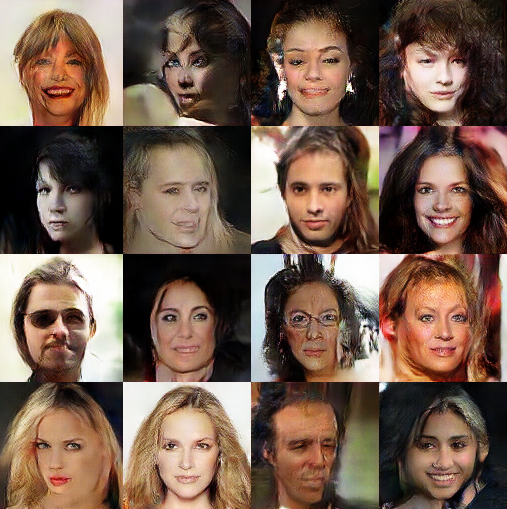
\includegraphics[width=\textwidth]{figures/result_part_on.png}
        \caption{Test result turn on part training after 20 epoch}
        \label{part_on}
    \end{minipage}
        \hfill
    \begin{minipage}[t]{0.48\linewidth}
        \centering
        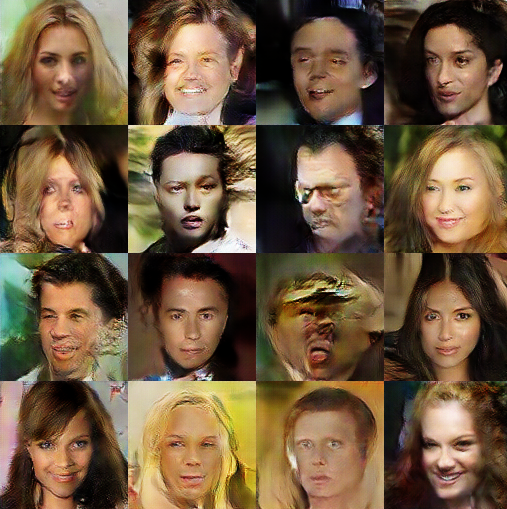
\includegraphics[width=\textwidth]{figures/result_part_off.png}
        \caption{Test result turn off part training after 20 epoch}
        \label{part_off}
    \end{minipage}
\end{figure}

\subsubsection*{Lower cost of the model}
We use a variety of methods to reduce the size of the model and reduce the amount of computation.
We compare the model size of pix2pix\upcite{pix2pix}, DCGAN\upcite{dcgan} and SmileGAN when outputting the same size image (a three-channel color image of 128 × 128 pixels).
(As shown in Figure \ref{result_model_size}).
It can be seen that the size of SmileGAN is smaller and SmileGAN costs less.

\begin{figure}
    \begin{center}
    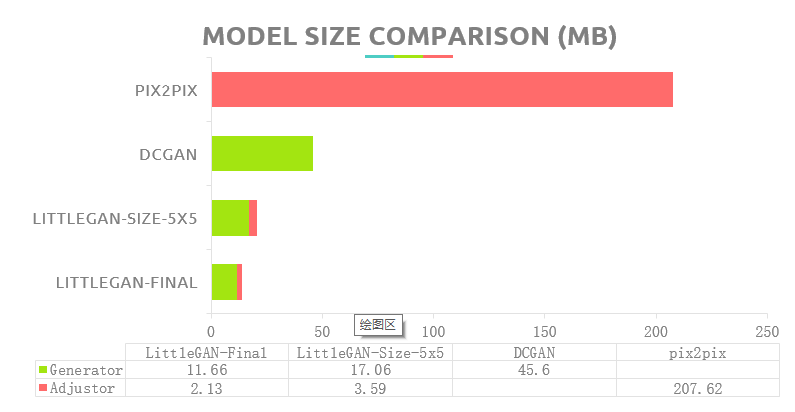
\includegraphics[width=\textwidth]{figures/result_model_size.png}
    \caption{Model Size Comparison}
    \label{result_model_size}
    \end{center}
\end{figure}